\documentclass[a4paper, 16pt]{article}
\usepackage[UTF8]{ctex}
\usepackage{geometry}
\usepackage{graphicx}
\usepackage{setspace}
\usepackage{float}
\usepackage{listings}
\usepackage{xcolor}
\lstset{
    numbers=left, 
    numberstyle= \tiny, 
    keywordstyle= \color{ blue!70},
    commentstyle= \color{red!50!green!50!blue!50}, 
    frame=shadowbox, % 阴影效果
    rulesepcolor= \color{ red!20!green!20!blue!20} ,
    escapeinside=``, % 英文分号中可写入中文
    xleftmargin=2em,xrightmargin=2em, aboveskip=1em,
    framexleftmargin=2em
} 
\geometry{left = 1.0 cm, right = 1.0cm, top = 2.0cm, bottom = 2.0cm	}
\title{编译原理第三章(二)}
\author{李鹏辉}

\begin{document}
\maketitle


1. 为下面语言设计一个DFA或NFA\\


1) 包含5个元音的所有小写字母串,这些串中元音按照顺序出现\\
\begin{figure}[H]
\centering
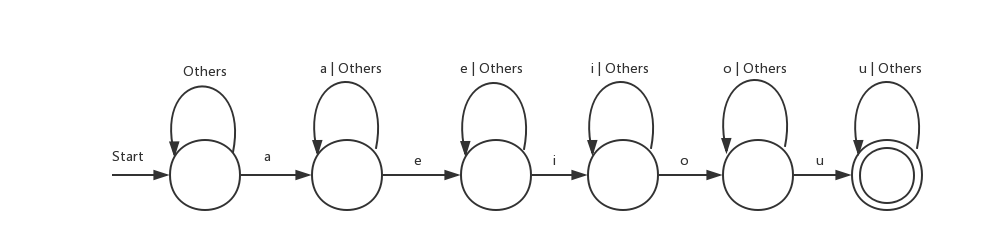
\includegraphics[scale = 0.6]{chapter3_hw2_1}
\caption{$Others = \{b | c |d | f| g| h | j | k | l | m | n| p | q | r| s| t| v| w| x| y|z \}$}
\label{f1}
\end{figure}
2) 所有由a,b组成得且不含子串abb的串\\
\begin{figure}[H]
\centering
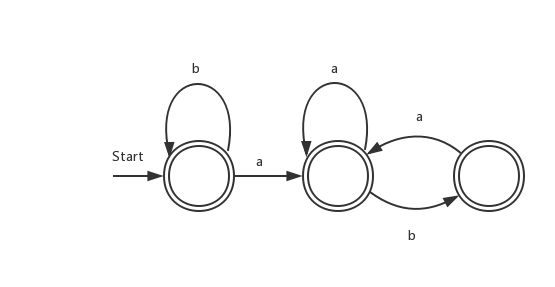
\includegraphics[scale = 0.6]{chapter3_hw2_2}
\caption{由a,b组成得且不含子串abb的串}
\label{f1}
\end{figure}
2. 用算法3.22模拟图3-29中得NFA在处理输入aabb时得过程.\\

	1)$S={0}; c = nextChar()  = a;$\\
	
	2)$c!= EOF \rightarrow S = \varepsilon-closure(move(S,a)) = \{0, 1\}, c = nextChar() = a$\\
	
	3) $c!= EOF \rightarrow S= \varepsilon-closure(move(S,a)) = \{0, 1, 2\}, c = nextChar() = b$\\
	
	4) $c != EOF \rightarrow S = \varepsilon-closure(move(s,b)) = \{0, 1, 2, 3\}, c = nextChar() = b$\\
	
	5) $c != EOF \rightarrow S = \varepsilon-closure(move(s,b)) = \{0, 1, 2, 3\}, c = nextChar() = EOF$\\
	
	6) $c == EOF \rightarrow S \cap F != \emptyset \: return \:yes$\\
	
3. 使用算法3.23和3.20将下述正则表达式转换为DFA,并尝试化简该DFA\\

1) $((\varepsilon|a)b^*)^*$\\
\begin{figure}[H]
\centering
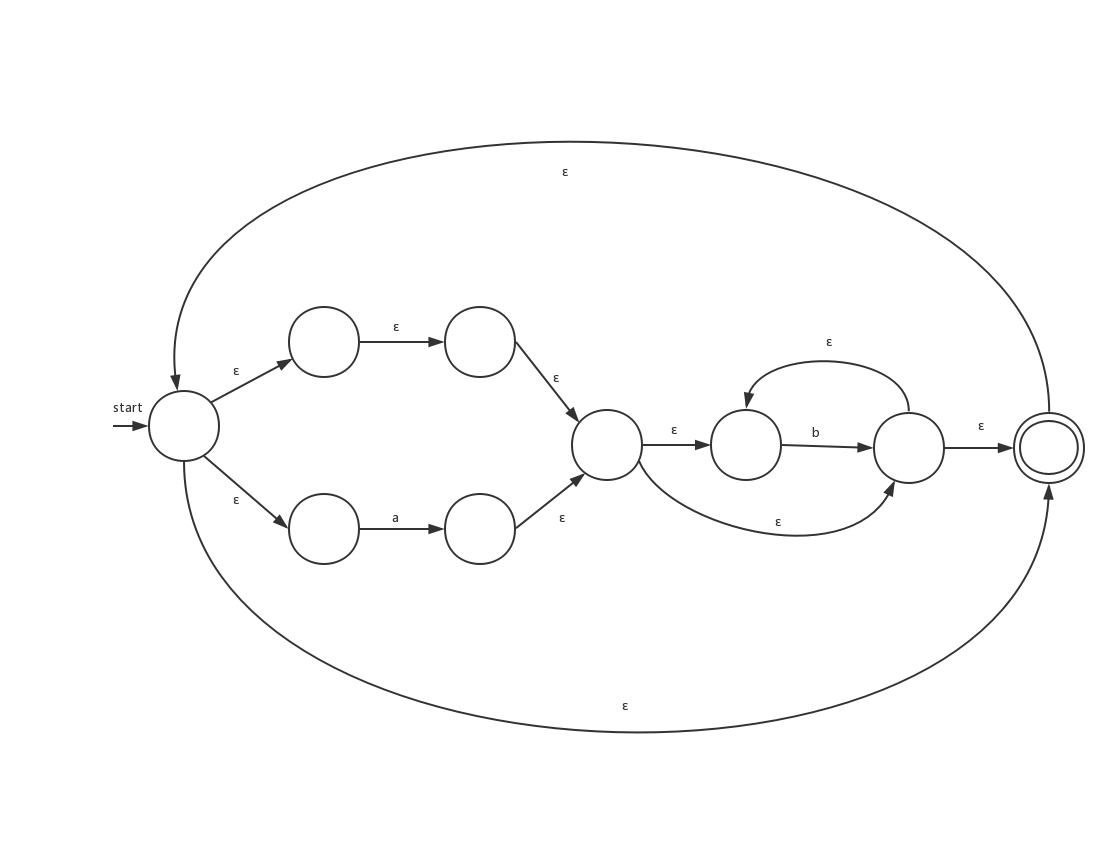
\includegraphics[scale = 0.4]{chapter3_hw2_3}
\caption{NFA$((\varepsilon|a)b^*)^*$}
\label{f1}
\end{figure}

\begin{figure}[H]
\centering
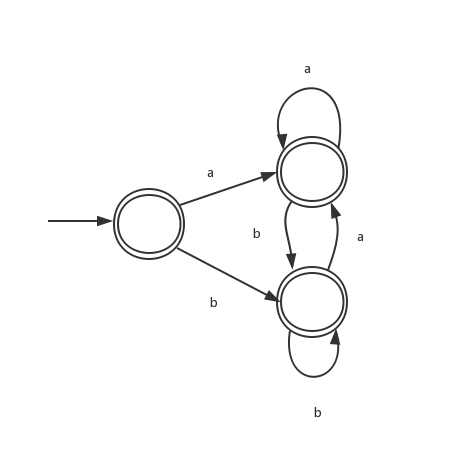
\includegraphics[scale = 0.6]{chapter3_hw2_4}
\caption{DFA$((\varepsilon|a)b^*)^*$}
\label{f1}
\end{figure}

\begin{figure}[H]
\centering
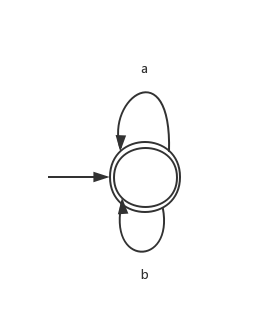
\includegraphics[scale = 0.6]{chapter3_hw2_7}
\caption{DFA化简$((\varepsilon|a)b^*)^*$}
\label{f1}
\end{figure}

2) $(a|b)^*abb(a|b)^*$\\
\begin{figure}[H]
\centering
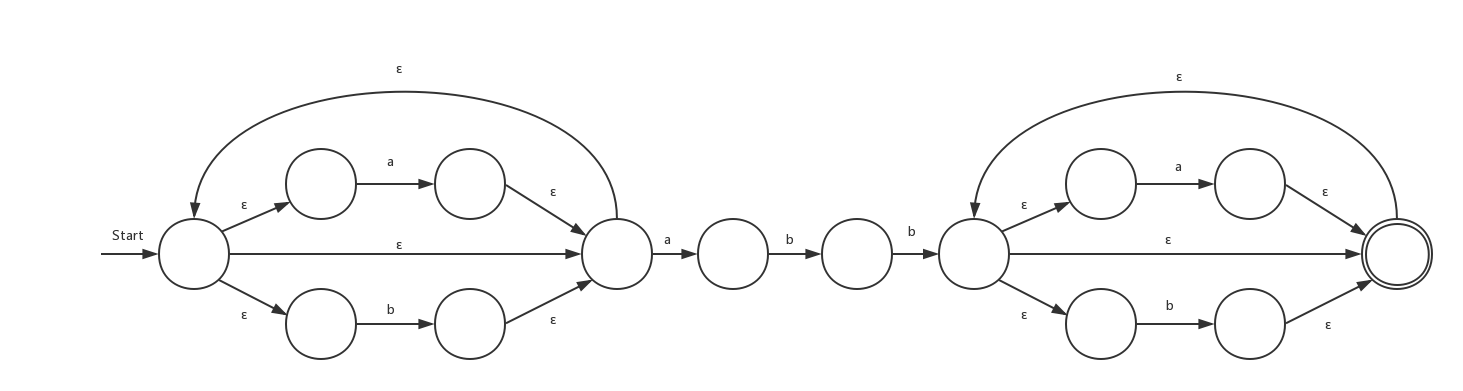
\includegraphics[scale = 0.3]{chapter3_hw2_5}
\caption{NFA$(a|b)^*abb(a|b)^*$}
\label{f1}
\end{figure}

\begin{figure}[H]
\centering
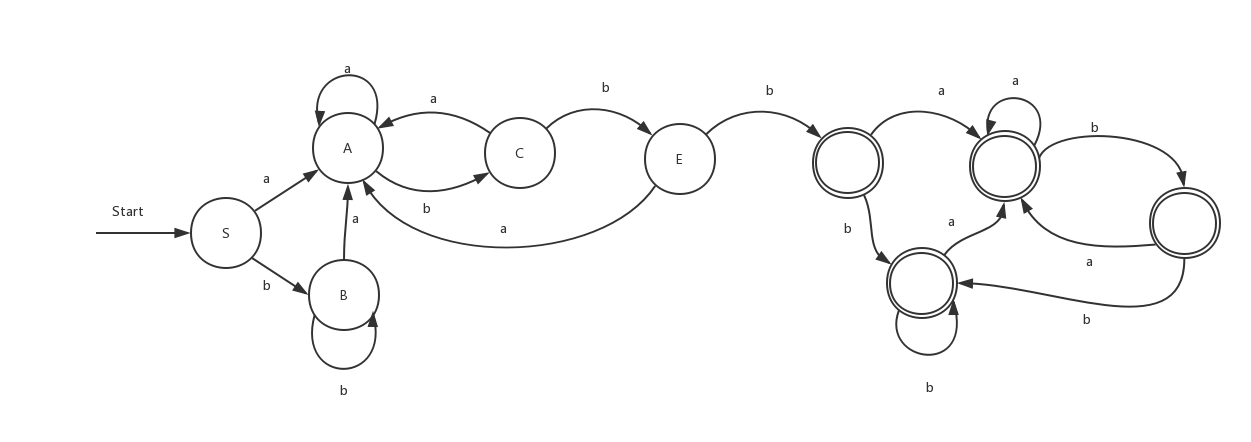
\includegraphics[scale = 0.4]{chapter3_hw2_6}
\caption{DFA$(a|b)^*abb(a|b)^*$}
\label{f1}
\end{figure}


\begin{figure}[H]
\centering
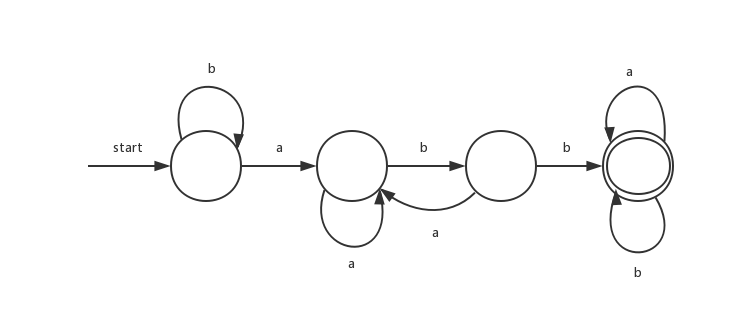
\includegraphics[scale = 0.5]{chapter3_hw2_8}
\caption{DFA化简$(a|b)^*abb(a|b)^*$}
\label{f1}
\end{figure}
\end{document}